\subsection{Product Functions}
%%%%%
%All the system features, i.e. all the functional requirements for the application
%%%%%
\subsubsection{State Diagrams of Product Functions}

\begin{center}
\textbf{The add user account function\\}
\end{center}
 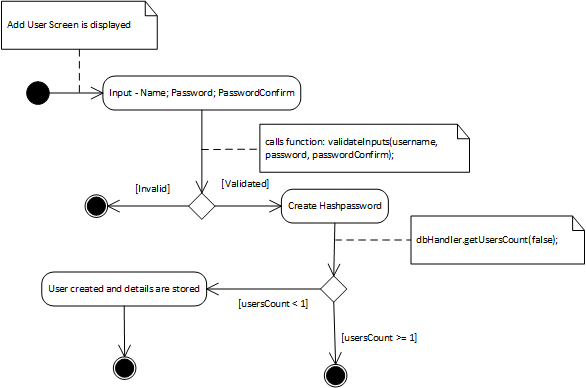
\includegraphics[width=13cm]{diagrams/StateDiagrams/AddUserStateDiagram.png}
\textbf{\\}
\begin{center}
\textbf{The Local Authentication function\\}
\end{center}
 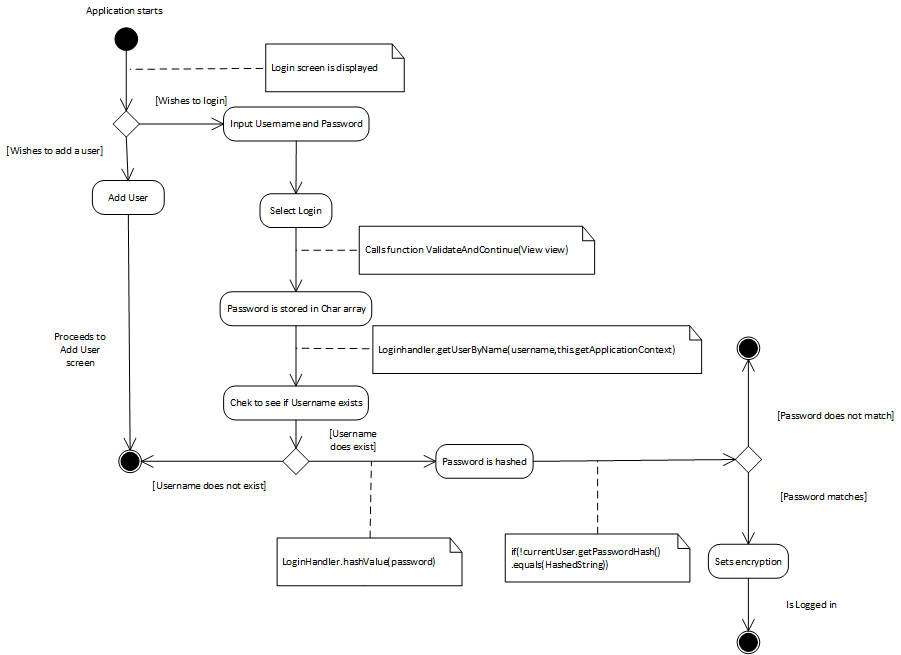
\includegraphics[width=13cm]{diagrams/StateDiagrams/LocalAuthenticationStateDiagram.png}
\textbf{\\}
\begin{center}
\textbf{The add contact function\\}
\end{center}
 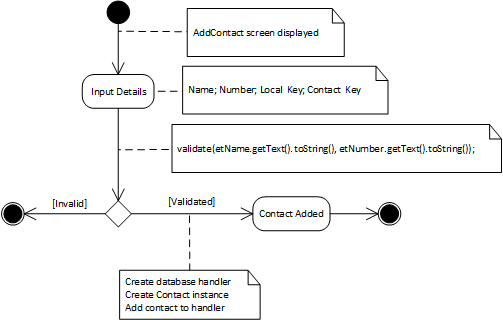
\includegraphics[width=13cm]{diagrams/StateDiagrams/AddContactStateDiagram.png}
\textbf{\\}
\begin{center}
\textbf{The edit contact function\\}
\end{center}
 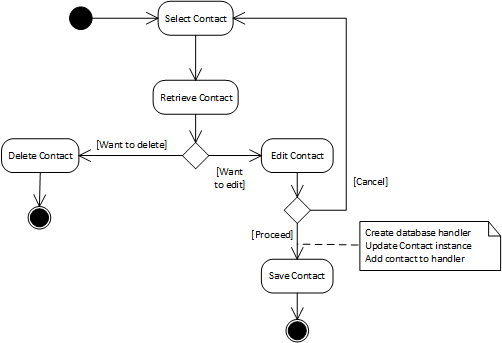
\includegraphics[width=13cm]{diagrams/StateDiagrams/EditContactStateDiagram.png}

\normalsize
\vspace{12pt}

\subsubsection{Admin Functions}
\begin{itemize}
\item{Add User Account : FRQ1}\\
\textbf{(Source: Bernard Wagner, Priority: Medium)}
\begin{itemize}
\item A user must be able to create a password protected account for the app.
\end{itemize}
%------------------------------------------------------------------------------------------------------------
\item{Edit User Password : FRQ2}\\
\textbf{(Source: Group Deliberation, Priority: Medium)}
\begin{itemize}
\item The user must be able to edit the authenticating password.
\end{itemize}
%------------------------------------------------------------------------------------------------------------
\item{Local Authentication : FRQ3}\\%meaning functional requirement 3
\textbf{(Source: Bernard Wagner, Priority: Medium)}
\begin{itemize}
\item The application must authenticate a user by requiring a password in order to log into the application, in order to ensure confidentiality.
\end{itemize}
%------------------------------------------------------------------------------------------------------------
\end{itemize}

\subsubsection{Messaging Functions}
\begin{itemize}
\item{Enter message : FRQ4}\\%meaning functional requirement 1
\textbf{(Source: Bernard Wagner, Priority: High)}
\begin{itemize}
\item A user must be able to input text into the application.
\end{itemize}
%------------------------------------------------------------------------------------------------------------
\item{Type message : FRQ4.1}\\
\textbf{(Source: Bernard Wagner, Priority: High)}
\begin{itemize}
\item A user must be able to type text into the application.
\end{itemize}
%------------------------------------------------------------------------------------------------------------
\item{Paste message : FRQ4.2}\\
\textbf{(Source: Bernard Wagner, Priority: High)}
\begin{itemize}
\item A user must be able to paste an already constructed message into the application, using the clipboard.
\end{itemize}
%------------------------------------------------------------------------------------------------------------
\item{Edit Message: FRQ5}\\
\textbf{(Source: Bernard Wagner, Priority: Medium)}
\begin{itemize}
\item The message text must be editable once it has been input into the application by the user.
\end{itemize}
%------------------------------------------------------------------------------------------------------------
\item{Encrypt message : FRQ6}\\
\textbf{(Source: Bernard Wagner, Priority: High)}
\begin{itemize}
\item The message must be encrypted using a suitable encryption method.
\end{itemize}
%------------------------------------------------------------------------------------------------------------
\item{Copy Encrypted Message : FRQ7}\\
\textbf{(Source: Bernard Wagner, Priority: High)}
\begin{itemize}
\item Once a message has been encrypted, a user must be able to copy the ciphertext, and paste it into a suitable messaging application.
\end{itemize}
%------------------------------------------------------------------------------------------------------------
\item{Decrypt message : FRQ8}\\
\textbf{(Source: Bernard Wagner, Priority: High)}
\begin{itemize}
\item The application must be able to decrypt the message (on the receiving end) to reveal the original text.
\end{itemize}
%------------------------------------------------------------------------------------------------------------
\item{Display message length : FRQ9}\\
\textbf{(Source: Bernard Wagner, Priority: Low)}
\begin{itemize}
\item The numbers of characters in the message must be displayed.
\end{itemize}
%------------------------------------------------------------------------------------------------------------
\end{itemize}

\subsubsection{Contacts Functions}
\begin{itemize}
\item{Add Contact : FRQ10}\\
\textbf{(Source: Bernard Wagner, Priority: High)}
\begin{itemize}
\item Before communicating with someone, the receiver must be added as a contact, in order to be able to communicate with that user.
\end{itemize}
%------------------------------------------------------------------------------------------------------------
\item{Edit Contact : FRQ11}\\
\textbf{(Source: Bernard Wagner, Priority: Medium)}
\begin{itemize}
\item A contact must be editable once it has been added.
\end{itemize}
%------------------------------------------------------------------------------------------------------------
\item{Remove Contact : FRQ12}\\
\textbf{(Source: Bernard Wagner, Priority: High)}
\begin{itemize}
\item A user must be able to remove a contact.
\end{itemize}
%------------------------------------------------------------------------------------------------------------
\end{itemize}

\subsection{i* Diagrams}
\subsubsection{General i* diagram}
SMSEncryption General i* diagram

\begin{center}
 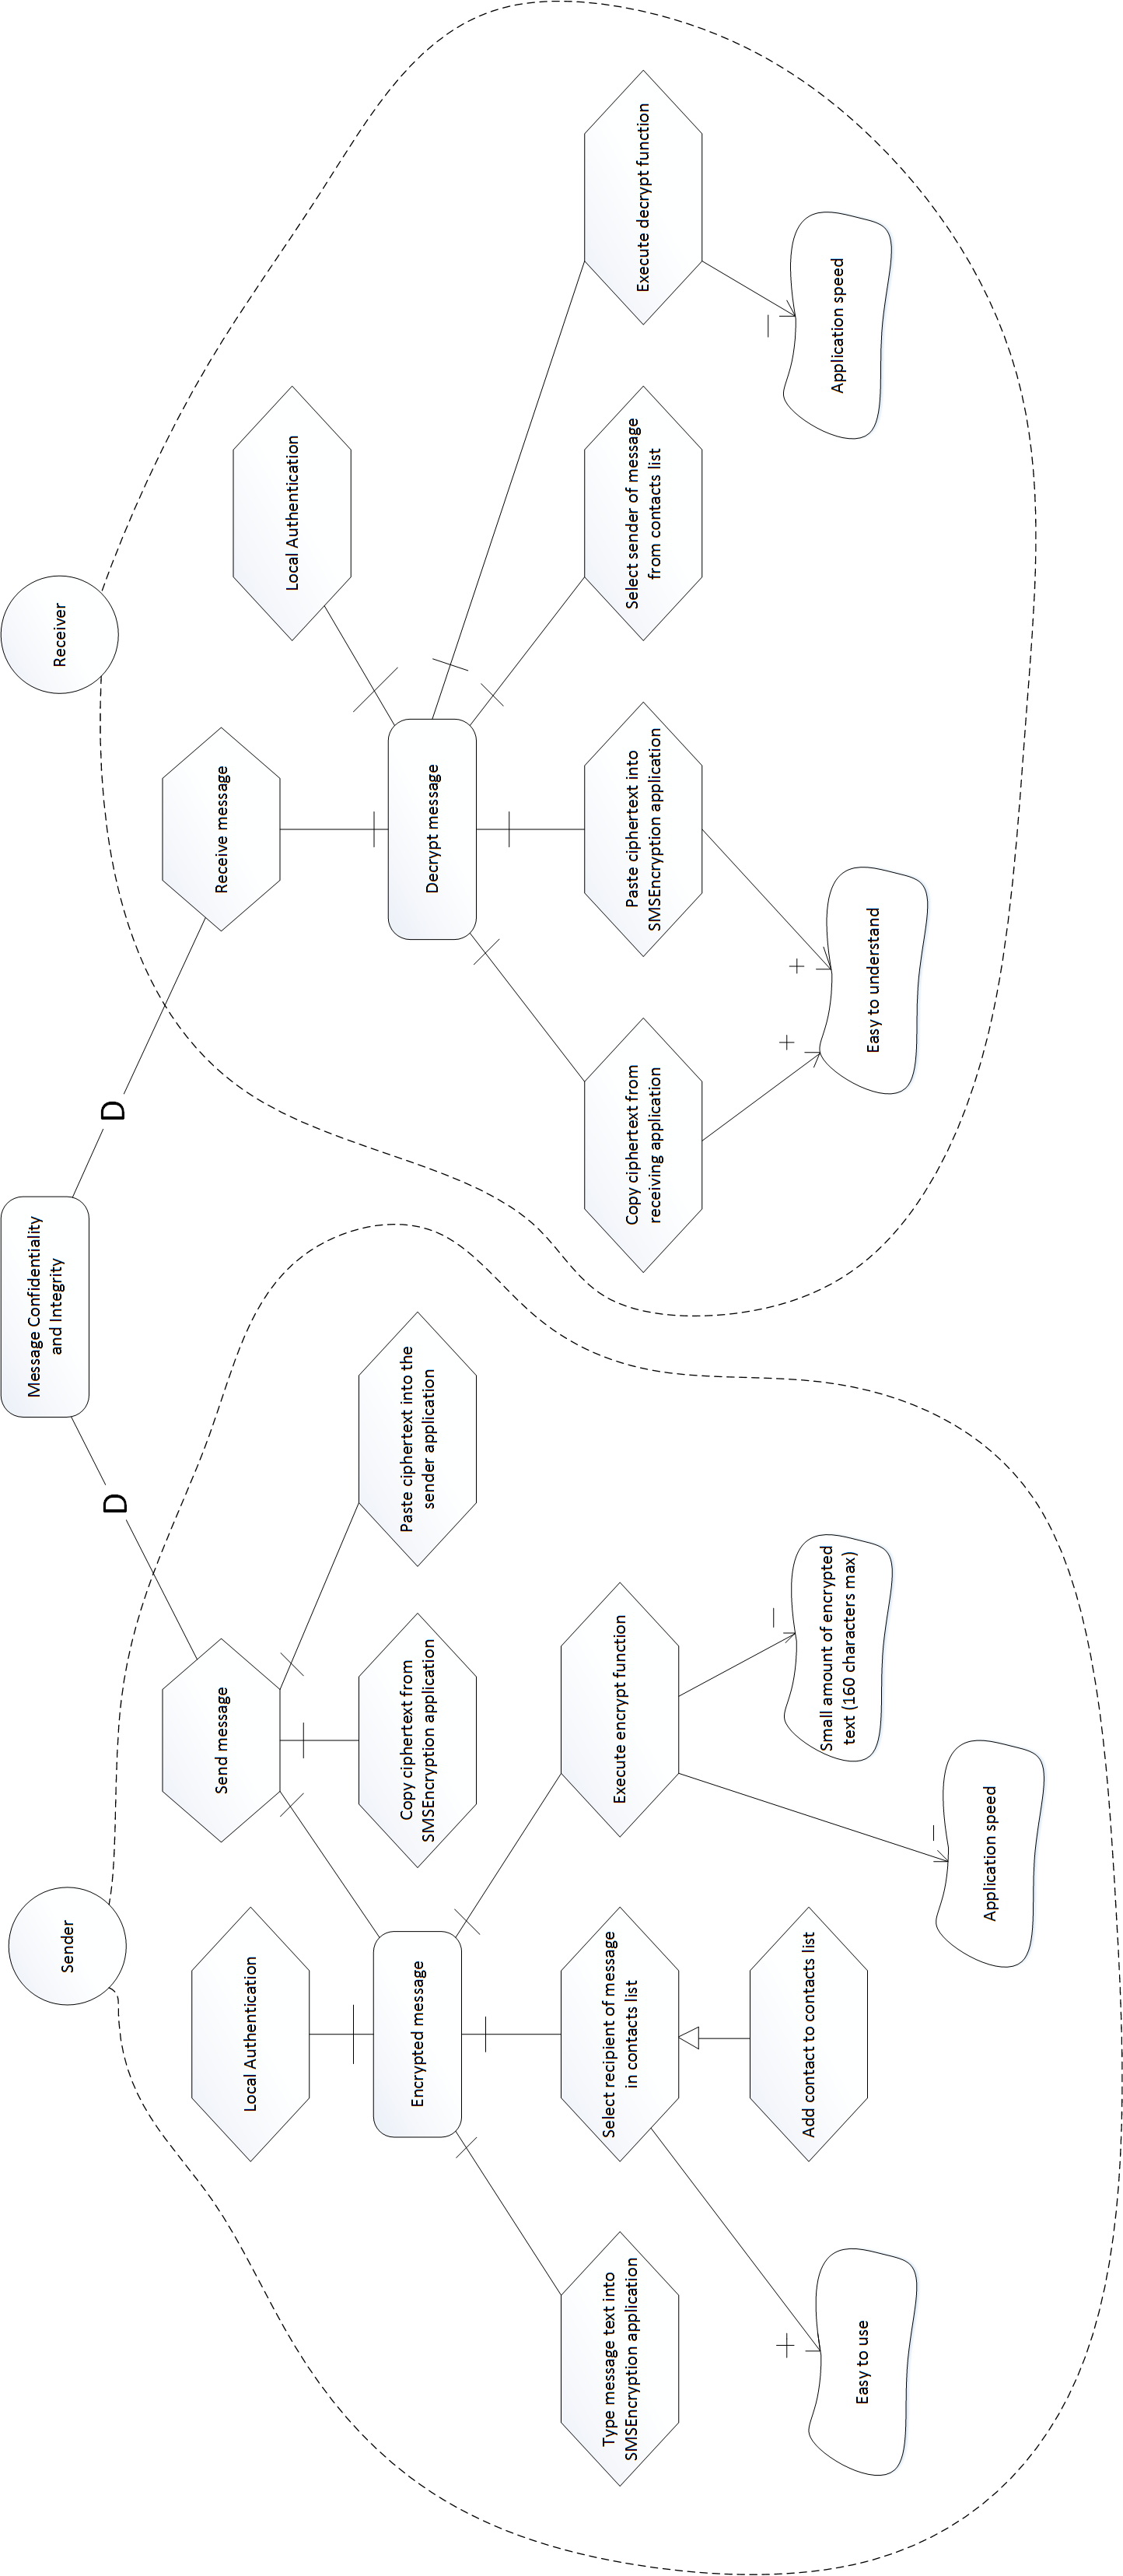
\includegraphics[height=21cm]{diagrams/IStarDiagrams/SMSEncryptionIStarDiagram.png}
\end{center}
